% coding:utf-8

%FOSAET, a LaTeX-Code for a electrical summary of basic electronics
%Copyright (C) 2013, Daniel Winz, Ervin Mazlagic

%This program is free software; you can redistribute it and/or
%modify it under the terms of the GNU General Public License
%as published by the Free Software Foundation; either version 2
%of the License, or (at your option) any later version.

%This program is distributed in the hope that it will be useful,
%but WITHOUT ANY WARRANTY; without even the implied warranty of
%MERCHANTABILITY or FITNESS FOR A PARTICULAR PURPOSE.  See the
%GNU General Public License for more details.
%----------------------------------------

\section{Strom und Spannung an Bauteilen}

\subsubsection{Widerstand}
\begin{figure}[h!]
	\centering
	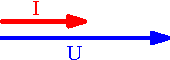
\includegraphics[width=0.3\textwidth]{zeig_ui_wid.pdf}
	\caption{Widerstand}
	\label{fig:zeig_ui_wid}
\end{figure}

\subsubsection{Kondensator}
\begin{figure}[h!]
	\centering
	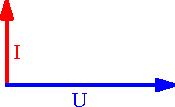
\includegraphics[width=0.3\textwidth]{zeig_ui_kap.pdf}
	\caption{Kondensator}
	\label{fig:zeig_ui_kap}
\end{figure}

\subsubsection{Spule}
\begin{figure}[h!]
	\centering
	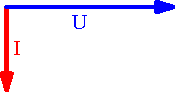
\includegraphics[width=0.3\textwidth]{zeig_ui_ind.pdf}
	\caption{Spule}
	\label{fig:zeig_ui_ind}
\end{figure}
